\documentclass{article}

\usepackage{color}
\usepackage{fullpage}
\usepackage{graphicx}
\usepackage{multicol}
\usepackage{multirow}
\usepackage{outline}
\usepackage{url}

\newcommand{\FIXME}[1]{\textcolor{blue}{[\textbf{FIXME}: {#1}]}}

\twocolumn


\title{Tweedr: Mining Twitter to inform Disaster Response}
\author{Zahra Ashktorab \and Chris Brown \and Jit Nandi \and Aron Culotta}


\begin{document}
\maketitle

\section{Introduction}

In recent years, Twitter has become a major channel for communication during
natural disasters. From \#snowpocalypse to \#Sandy, Twitter users have shared
news, photos and observations from the midst of hurricanes, blizzards,
earthquakes and other emergencies. First responders can utilize these streams
of data generated by social media to find out where the disasters are
happening and what specifically has been effected as a result of it.  As with
most social media conversations, informative signals are often drowned out by
irrelevant and redundant noise. First responders struggle to glean actionable
knowledge from the flood of tweets and status updates.

In order to solve this problem, we propose {\tt tweedr}: Twitter for Disaster
Response.\footnote{\url{http://tweedr.dssg.io}} The goal of this tool is to
extract information relevant for first responders from tweets generated during
disasters. The {\tt tweedr} pipeline consists of three main parts:
classification, clustering and extraction. In the classification phase, we use
a variety of classification methods (sLDA, SVM, and LogReg) to classify
whether a tweet reports disaster damage or casualty information. In the
clustering phase, we utilize filters to merge tweets that are similar to one
another; and finally in the extraction phase, we extract specific tokens and
phrases that report specific information about different classes of
infrastructure damage, damage types, and casualties. Using these three phases,
the Tweedr pipeline is able to extract actionable information from a stream of
tweets during disasters.

\section{Data}

We identified 12 crisis events that occurred in North America since the
founding of Twitter in 2006. We then constructed queries to collect relevant
tweets from Gnip, a social media aggregation company. We constructed two types
of queries: (1) keyword ({\bf kw}) queries contain search terms and hashtags
determined to be relevant based on a post-hoc analysis; (2) geographical
queries ({\bf geo}) consisting of a bounding box of coordinates around the
epicenter of the event. Table \ref{tab.data_summary} lists the number of
tweets collected for each event.

We can see considerable variation in the number of messages for each
crisis. This is in part explained by the popularity of Twitter overall, the
number of people affected, and by Twitter usage in the affected
area. Additionally, more recent events return more matches for the
geographical queries -- this follows from the increased usage of geolocation
services on Twitter.

\begin{table*}
\centering
\small
\begin{tabular}{|l|r|r|r| p{8cm} |}
\hline
{\bf Event}  & {\bf N (kw)} & {\bf N (geo)} & {\bf total} & {\bf keywords} \\
\hline
christchurch &  759,399  & 2,017       &  761,416    & \#EQNZ,\#CHCH,\#NZquake,Christchurch\\
ike          &  113,773  & 3,989       &  117,762    & Hurricane+Ike,Hurricane,Ike,Galveston,Houston\\
irene        &  384,689  & 3,871,631   &  4,256,320  & \#Hurricane,\#Irene,\#Tropics\\
moore        &  842,318  & 1,579,056   &  2,421,374  & \#mooretornado,\#moore,newcastle\\
oklahoma     & 1,697,891 & 6,209,510   &  7,907,401  & \#oklahoma,\#tornado,\#oklahomatornado,\#okwx,\#okc\\
samoa        & 235,208   &  2,016      &  237,224    &  Samoa,tsunami,earthquake\\
slavelake    & 45,072    &  1,281      &  46.353     & \#SlaveLake,Slave+Lake\\
supertuesday & 22,205    &  2,201      &  24,406     & Super+Tuesday,Jackson,Memphis,supertuesday\\
tornado2011a & 476,730   &  2,293      &  479,023    & Tushka,oklahoma,okwx,arkansas,akwx,tornado\\
tornado2011b & 52,201    &  2,326      &  54,527     & \#alwx,\#okwx,\#txwx,\#tristatewx,tornado,\mbox{\#ALNeeds}, \#ALHaves,\#WeAreAlabama\\
vtech        & 16,652    &  2,869      &  19,521     & \#vatech,\#virginiatech,\#hokies,\#vtech,\#vt\\
westtx       & 651,045   &  178,846    &  829,891    & \#WestExplosion,\#WestTX\\
\hline
{\bf Total}  & {\bf 5,297,183} & {\bf 11,858,035}  & {\bf 17,155,218}  &\\
\hline
\end{tabular}
\caption{Number of tweets collected by event. We query for tweets both by
  keyword ({\bf kw}) and geographical bounding box ({\bf geo}). \label{tab.data_summary}}
% See dssg-twitter-disaster/aron/count_lines.py
\end{table*}

\subsection{Data Annotation}
To train and evaluate our automated methods, we must first collect
human-annotated examples. We consider two tasks for annotation:
\begin{enumerate}
  \item {\bf Classification}: Does the tweet mention either specific
    infrastructure damage or human casualty? We treat this as a binary
    classification task. Positive examples include ``10 injured in plant
    explosion'' and ``The windows are smashed at the Whole Foods on 1st'';
    however, ``Hurricane Irene causes massive damage'' would be a negative
    example, since it does not include specific, actionable damage
    information.
  \item {\bf Extraction}: For positive examples of the above, identify the
    tokens in the tweet corresponding to specific types of infrastructure
    damage or counts of the number of dead or injured. For example, in the
    tweet ``Flooding bad up and down sides of Green River Rd,'' the token
    ``Flooding'' should be annotated as a damage type, and the tokens ``Green
    River Rd'' should be labeled as a road. The full ontology is listed in
    Table \ref{tab.by_label}.
\end{enumerate}

Since not all data can be labeled manually, we sample a small subset. Half of
the tweets are selected uniformly at random from each event; the remaining
half are sampled from tweets matching a set of keywords heuristically
determined to be relevant to our task.\footnote{The keywords are: bridge,
  intersection, car, bus, truck, vehicle, evacuation, evacuate, fire, police,
  institution, wind, impact, injured, damage, road, airplane, hospital,
  school, home, building, flood, collapse, death, casualty, missing.} We do
this to mitigate the class imbalance problem (i.e., most tweets are not
relevant to infrastructure damage or casualties).

We sampled 1,049 tweets of the resulting tweets, of which 793 were labeled as
positive examples. We then annotate the extraction labels for each positive
example.
% mysql> select count(*) from DamageClassification where mturk_code='QCRI';
% 1049
% mysql> select count(*) from DamageClassification where mturk_code='QCRI' and Infrastructure=1 or Casualty=1;
% 793


\section{Experiments}

\subsection{Classification}
We compare a number of standard classification algorithms, including
$K$-nearest neighbors, decision trees, na\"ive Bayes, and logistic regression,
as implemented in the {\tt scikit-learn} Python
library.\footnote{\url{http://http://scikit-learn.org/}} We also compare with
supervised latent Dirichlet allocation~\cite{blei10supervised}, for which we
create a Python wrapper of the R {\tt lda}
package.\footnote{\url{http://cran.r-project.org/web/packages/lda/}}

Table \ref{tab.classification_results} displays the accuracy of each
method. Logistic regression appears to be the most reliable across several
accuracy measures.


\begin{table*}[t]
\centering
\begin{tabular}{|c|c|c|c|c|c|}
\hline
{\bf Method}  &  {\bf F1}        &  {\bf Pr}       &  {\bf Re}       & {\bf Acc}       &  {\bf AUC}\\
\hline
{\bf LogReg}  & {\bf .65 $\pm$ .07}& .78 $\pm$ .08       &  .57 $\pm$ .09       & {\bf .86 $\pm$ .03}& {\bf .88} \\
{\bf NB}      & .63 $\pm$ .06      & .55 $\pm$ .07       &  .{\bf 75 $\pm$ .09} & .80 $\pm$ .03      & .84 \\
{\bf DTree}   & .54 $\pm$ .09      & {\bf .93 $\pm$ .07} &  .39 $\pm$ .09       & .85 $\pm$ .02      & .69 \\
{\bf KNN}     & .51 $\pm$ .04      & .83 $\pm$ .10       &  .38 $\pm$ .04       & .84 $\pm$ .02      & .73 \\
{\bf sLDA}    & .50 $\pm$ .07      & .42 $\pm$ .06       &  .65 $\pm$ .15       & .70 $\pm$ .05      & .77 \\
\hline
\end{tabular}
\caption{Damage/casualty classification results (with standard
  deviations). {\bf Pr:} precision, {\bf Re:} recall, {\bf Acc:} accuracy,
  {\bf AUC:} area under the ROC curve. \label{tab.classification_results}}
\end{table*}


\subsection{Extraction}
For extraction, we use a conditional random field (CRF)~\cite{sutton12intro}, as
implemented by the {\tt CRFsuite}
toolkit.\footnote{\url{http://www.chokkan.org/software/crfsuite/}}. We consider several different types of features for our CRF. For each token in a tweet, we inspect capitalization, pluralization, whether it is numeric or includes a number, whether it is part of a determined lexicon of transportation types or building types, hypernyms, ngrams, and part of speech tags. 
To obtain precision, recall, and F1-score values, we split the data using two methods. In Table \ref{tab.by_label}, we use 10-folds cross validation. Additionally, we split the data by disaster, training on the labeled data from our top 5 disaster and testing on the sixth. The disasters we trained on this second method include: Joplin, Irene, Samoa, Christchurch, Tornado2011b, and Oklahoma. By splitting the training and testing data on disaster, we can test the accuracy of our classifier on unseen disasters. In Table \ref{tab.unseen_disaster}, we show the overall average for the CRF for performing on an unseen disaster.

As seen by Table \ref{tab.by_label}, our entity extraction classifier performs well (obtains an F1-score above .5) on predicting missing persons, religious institutions, electricity loss, hospital and health infrastructures, death/casualties, and wind/projectile damage. However, it does not predict fires and homes/residential infrastructures as accurately as the aforementioned labels. Furthermore, due to the nature of content in tweets, there is insufficient labeled data for certain labels and thus precision, recall and F1-scores could not be obtained.
We also evaluated our CRF across disasters to evaluate how it performed on disasters it had not seen yet. The results were promising for some disasters, yielding promising F1-score values for four of the six disasters evaluated. The results are reflected in Table \ref{tab.unseen_disaster}. Additionally, the confusion matrix in Figure \ref{cm} shows some misclassification between wind damage and death/casualties -- both types of messages often contain numerical tokens (e.g., ``100s people wounded'' versus ``100s of downed trees'').


\subsection{Clustering}
We consider two different methods of approximate string matching: Bloom
filters~\cite{bloom70space} and SimHash~\cite{charikar02similarity}. We have
not yet performed any quantitative evaluation of these approaches -- we leave this
for future work.


\begin{table}[t]
\centering
\small
\begin{tabular}{|l|r|r|r| p{8cm} |}
\hline
{\bf Label}  & {\bf F1} & {\bf Pr} & {\bf Re} \\
\hline
missing persons &  0.86  & 0.80       &  1.00 \\
religious institution          &  0.68  &    0.63    &  0.75\\
other damage        &  0.63  & 0.52   &  1.00\\
other building        &  - & -  &  -\\
electricity loss     & 0.88 & 0.81   &  1.00\\
snow        & - & - & - \\
evacuation center    &  - &  -   &  - \\
hospital/health services & 0.76 & 0.71 & 0.96 \\
other transportation & - & - & - \\
intersection & - & - & - \\
road        & - & - & - \\
bridge       & - & - &  -\\
homes/residential    & 0.47 & 0.33 &  1.00\\
fire & 0.33 & 0.20 & 1.00 \\
school & - & - & - \\
fire/police department & - & - & - \\
building collapse        & - & - & - \\
injured person & - & - & - \\
bus & -   &  -    &  -\\
airplane & -  &  -  &  -\\
death/casualties & 0.60  &  0.44  &  0.96\\
wind/projectile damage & 0.75  &  0.65   &  0.90\\
flood & -   &  -  &  -\\
vehicular impact & -   &  -    &  -\\
\hline
{\bf Average}  & {\bf 0.47} & {\bf 0.32}  & {\bf 0.88}  \\
\hline
\end{tabular}
\caption{Extraction F-score, Precision, and Recall values for each
  label. Missing values occur because many label types in our ontology did not
  appear in the data. \label{tab.by_label} }
\end{table}

\begin{table}[t]
\centering
\small
\begin{tabular}{|l|r|r|r| p{8cm} |}
\hline
{\bf Disaster}  & {\bf F1} & {\bf Pr} & {\bf Re} \\
\hline
Joplin &  0.79  & 0.65       &  1.00 \\
Irene          &  0.13  &    0.11    &  0.714\\
Samoa        &  1.00  & 1.00   &  1.00\\
Christchurch        &  -  & - & - \\
Tornado 2011b     & 1.00 & 1.00   &  1.00\\
Oklahoma       & 0.44 & 0.29 & 1.00 \\
\hline
{\bf Average}  & {\bf 0.60} & {\bf 0.49}  & {\bf 0.77}  \\
\hline
\end{tabular}
\caption{Extraction F-score, Precision, and Recall obtained by training on 5
  disasters and testing on the sixth. This assesses the ability of the
  algorithm to generalize to new disasters. \label{tab.unseen_disaster} }
\end{table}

\begin{figure}[ht!]
\centering
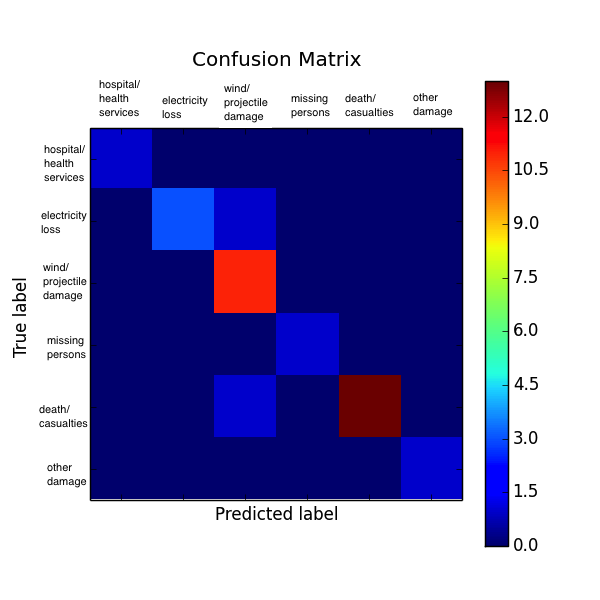
\includegraphics[width=90mm]{confusion_matrix}
\caption{Confusion Matrix of predicted labels using 10-folds cross validation. \label{cm}}
\end{figure}

% FIXME:
%\begin{table}[t]
%\centering
%\begin{tabular}{|l|}
%\hline
%{\bf Correctly identified as damage or casualty}\\
%\hline
%xxxx\\
%\hline
%{\bf Incorrectly identified as damage or casualty}\\
%\hline
%xxxx\\
%\hline
%\end{tabular}
%\end{table}

\section{Related Work}
There has been growing interest in using social media for situational
awareness during a
disaster~\cite{kumar_tweettracker_2011,cheong_social_2011,mandel12demo,meier_extracting_2013,imran_practical_2013}. Our
work builds upon that of Imran et al.~\cite{imran_practical_2013}, who also
use a CRF to extract damage and casualty information from tweets. Our main
contributions are experiments with an expanded ontology, feature set, and
set of events.


\section{Conclusions and Future Work}
We have outlined initial experiments using {\tt Tweedr} to extract relevant
information from tweets during a disaster. Additional experiments are needed
to understand the behavior of these methods in real-world, dynamic
environments. Also, given the low frequency of relevant tweets, methods
designed for high class imbalance~\cite{lin_class-imbalanced_2012} may be
useful here.

\section{Acknowledgments}
This work was performed during the 2013 Eric \& Wendy Schmidt Data Science for
Social Good Fellowship at the University of Chicago, in partnership with the
Qatar Computational Research Institute. We are grateful to Gnip for providing
access to the historical tweets used in this analysis, as well as to all the
2013 DSSG Fellows who helped with data annotation.

\bibliographystyle{abbrv}
\bibliography{tweedr}

\end{document}




